\documentclass{article}
\usepackage[T1]{fontenc}
\usepackage{lmodern}
\usepackage{graphicx}
\usepackage{amsmath,amssymb}
\usepackage[a4paper,margin=2cm]{geometry}
\usepackage[absolute,overlay]{textpos}
\setlength{\TPHorizModule}{1mm}
\setlength{\TPVertModule}{1mm}
\usepackage[indonesian]{babel}
\usepackage{hyperref}
\setlength{\emergencystretch}{2em}
% unit: Halaman 93

\begin{document}

% === Halaman 93 (llm) ===

\vspace{279.18mm}

Sumber: Wikipedia

% deskripsi: Implementasi kode program C untuk algoritma ChaCha20, mencakup makro ROTL, makro QR (Quarter Round), dan fungsi chacha\_block.
% bbox normalisasi: [0.0100, 0.0200, 0.9700, 0.9600]
\begin{textblock*}{201.60mm}(2.10mm,5.94mm)
\noindent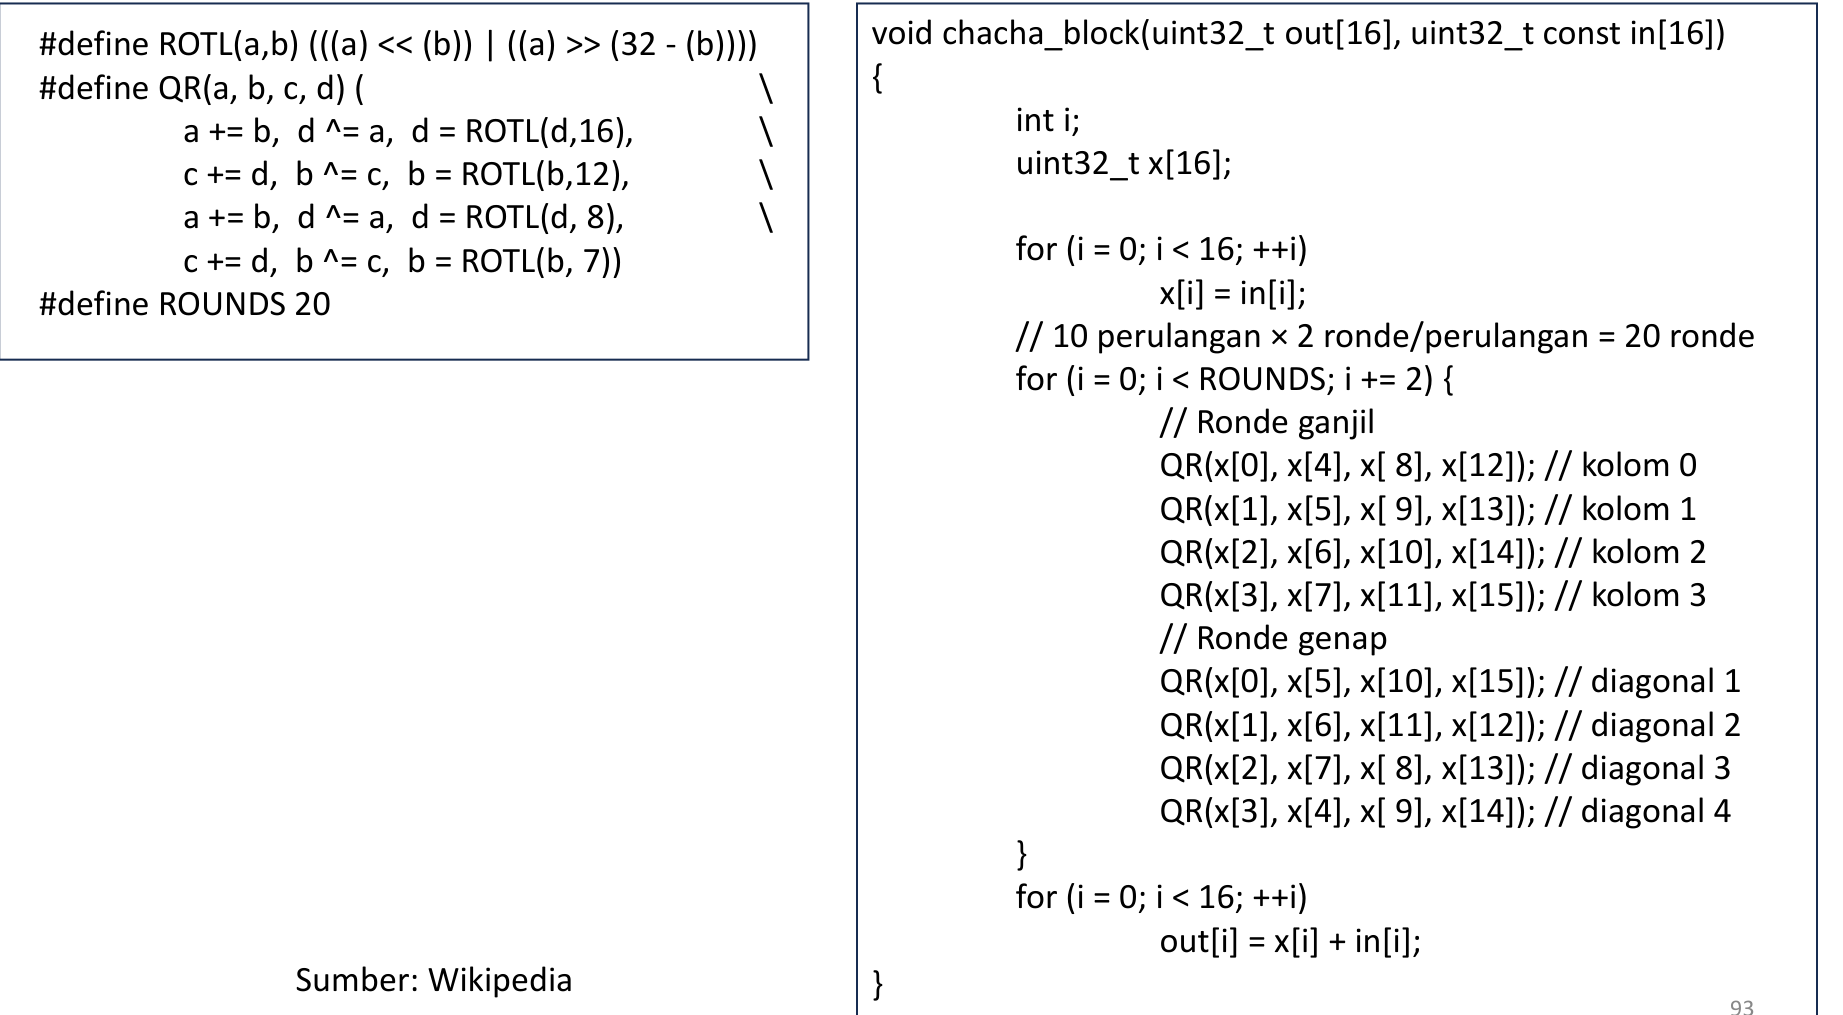
\includegraphics[width=201.60mm,height=279.18mm]{../../images/llm/page_093_img_01.png}%
\end{textblock*}

\end{document}
